\documentclass[12pt, twoside]{article}
\usepackage[letterpaper, margin=1in, headsep=0.5in]{geometry}
\usepackage[english]{babel}
\usepackage[utf8]{inputenc}
\usepackage{amsmath}
\usepackage{amsfonts}
\usepackage{amssymb}
\usepackage{tikz}
%\usetikzlibrary{quotes, angles}

\usepackage{graphicx}
\usepackage{enumitem}
\usepackage{multicol}

\usepackage{fancyhdr}
\pagestyle{fancy}
\fancyhf{}
\renewcommand{\headrulewidth}{0pt} % disable the underline of the header

\fancyhead[LE]{\thepage}
\fancyhead[RO]{\thepage \\ Name: \hspace{4cm} \,\\}
\fancyhead[LO]{BECA / Dr. Huson / Geometry\\* Unit 7: Similarity\\* 3 January 2020}

\begin{document}
\subsubsection*{7.2 Do Now: Slope and the tangent function, similar triangles}
  \begin{enumerate}
  \item \begin{enumerate}
    \item Graph and label $\triangle ABC$ with $A(0,0)$, $B(7,4)$, and $C(7,0)$.
    \begin{center}
      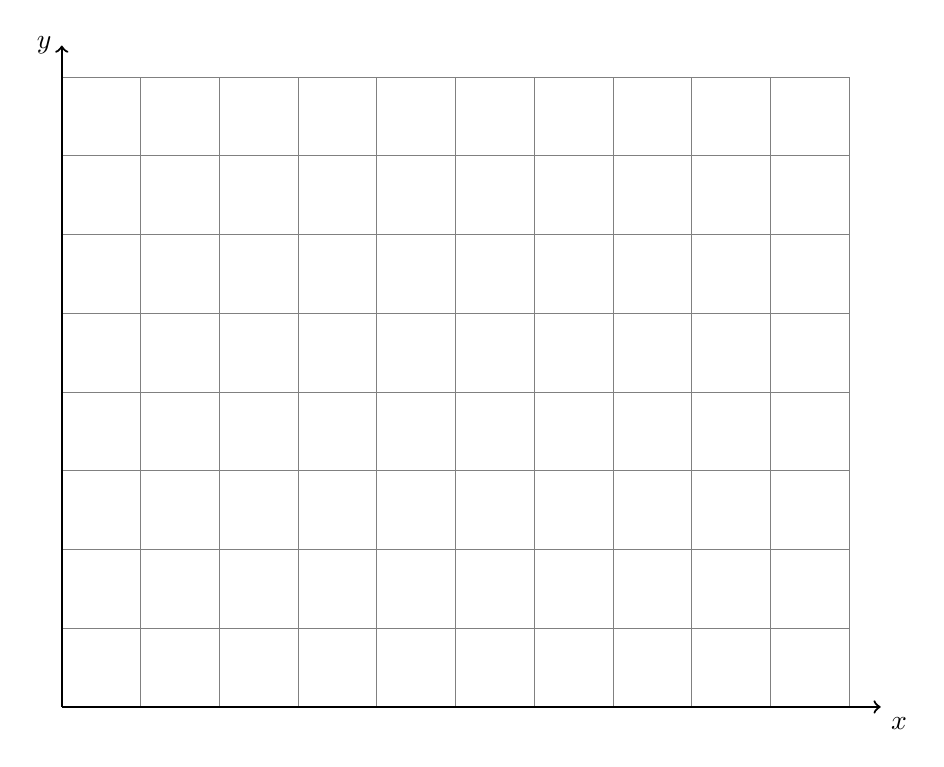
\begin{tikzpicture}%[scale=.635]
        \draw [help lines] (0,0) grid (10,8);
        \draw [thick, ->] (0,0) -- (10.4,0) node [below right] {$x$};
        \draw [thick, ->] (0,0)--(0,8.4) node [left] {$y$};
      \end{tikzpicture}
    \end{center}
    \item Find the slope and $y$-intercept of the line $\overleftrightarrow{AB}$.
      \begin{multicols}{2}
        $m_{AB}=$ \\
        $b_{AB}=$
      \end{multicols} \vspace{0.5cm}
    \item Write down the equation of each line. \\[0.5cm]
      $\overleftrightarrow{AB}$: \hfill
      $\overleftrightarrow{BC}$: \hfill
      $\overleftrightarrow{AC}$: \hspace{2cm}
    \vspace{2cm}
    \item Find the measure of $\angle BAC$ in degrees with a protractor. \vspace{0.5cm}
    \item Find the same $m\angle BAC$ with a calculator's inverse tangent function.\\[0.5cm]
    $\displaystyle \tan^{-1}(\frac{4}{7})=$
    \vspace{2cm}
  \end{enumerate}


\newpage
  \item Given $\triangle ABC$ has sides $AC = 6$, $BC = 5$, $AB = 4$. $\triangle ABC$ is reflected across the bisector of $\angle BAC$ and then dilated by a factor of $k=2$ centered at $A$, creating the image shown. Complete the similarity statement (with the letters in the right order) and calculate the lengths of the triangle image.
  \begin{multicols}{2}
    \begin{enumerate}
      \item $\triangle ABC \sim$ \vspace{0.3cm}
      \item $AZ=$ \vspace{0.3cm}
      \item $AX=$ \vspace{0.3cm}
      \item $XZ=$
    \end{enumerate}
        \begin{flushright}
        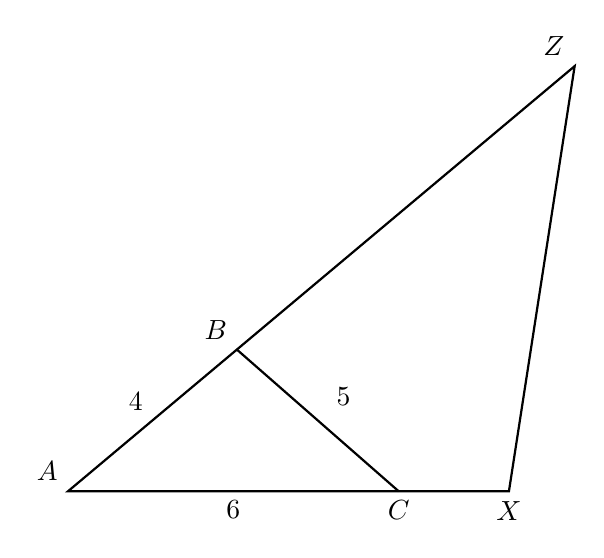
\begin{tikzpicture}[scale=0.7]
          \draw [-, thick] (0,0) node[above left]{$A$}--
          (0:8) node[below]{$X$}--
          (40:12) node[above left]{$Z$}--cycle;
          \draw [thick] (0:6)--(40:4);
          \node at (40:4) [above left]{$B$};
          \node at (0:6) [below]{$C$};
          \node at (40:2) [above left]{$4$};
          \node at (3, 0) [below]{$6$};
          \node at (20:5) [right]{$5$};
        \end{tikzpicture}
      \end{flushright}
    \end{multicols} \vspace{1cm}
  
  \item Given $\triangle ABC \sim \triangle AED$ and $AB = 11$, $BC = 8$, $AC = 15$, $DE=24$. \\[0.5cm] Find:
  \begin{multicols}{2}
    \begin{enumerate}
      \item $k=$ \vspace{0.3cm}
      \item $AD=$ \vspace{0.3cm}
      \item $AE=$ \vspace{0.3cm}
      \item $CE=$
    \end{enumerate}
        \begin{flushright}
        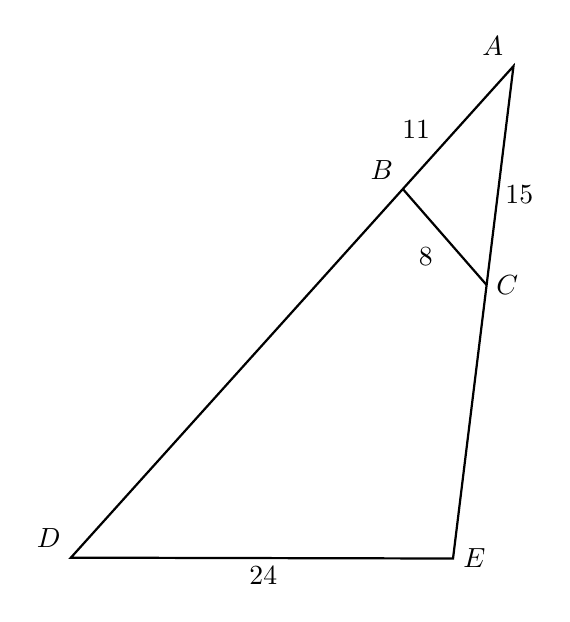
\begin{tikzpicture}[rotate=3, scale=0.7]
          \draw [-, thick] (0,0) node[above left]{$A$}--
          (-100:9) node[right]{$E$}--
          (-135:12) node[above left]{$D$}--cycle;
          \draw [thick] (-100:4)--(-135:3);
          \node at (-135:3) [above left]{$B$};
          \node at (-100:4) [right]{$C$};
          \node at (-135:2) [above left]{$11$};
          \node at (-90:2) [below]{$15$};
          \node at (-120:3.5) [below]{$8$};
          \node at (-120:10) [below]{$24$};
        \end{tikzpicture}
      \end{flushright}
    \end{multicols}

\end{enumerate}
\end{document}